\section{Configuration overview}
The mARGOt autotuning framework implements a Monitor-Analyze-Plan-Execute loop based on application knowledge (MAPE-K).
While the Analyze and Execute elements of the loop do not require any configuration, the  Monitor, Plan and Knowledge elements need some input from the user.
In particular, the Monitor element requires the user to specify the monitors of interest for the application and, for each monitor, the related statistical properties that must be exposed.
The Plan element need to know the definition of ``best'' configuration from the user, defined as a constrained multi-objective problem.
Finally, the application Knowledge should describe the application behavior, by varying the selected configuration.
In particular, the knowledge is a list of a paired information.
Each pair relates an application configuration with performance reached using that configuration.



The autotuner handles a single block of code of the application.
To match phases of the application, we might use more than one autotuner, where each instance handles a different block of code of the application. 
For this reason, the configuration of the MAPE-K elements of an autotuner, are related to a single block of code.
Moreover, to employ separation of concerns, the Knowledge of the application is split in a different file with respect to the other information.
For this reason we have one common configuration file for all the Monitor and Plan elements of each block of code of the application; but we have different files for the Knowledge of different blocks of code of the application.

\begin{figure}
\centering
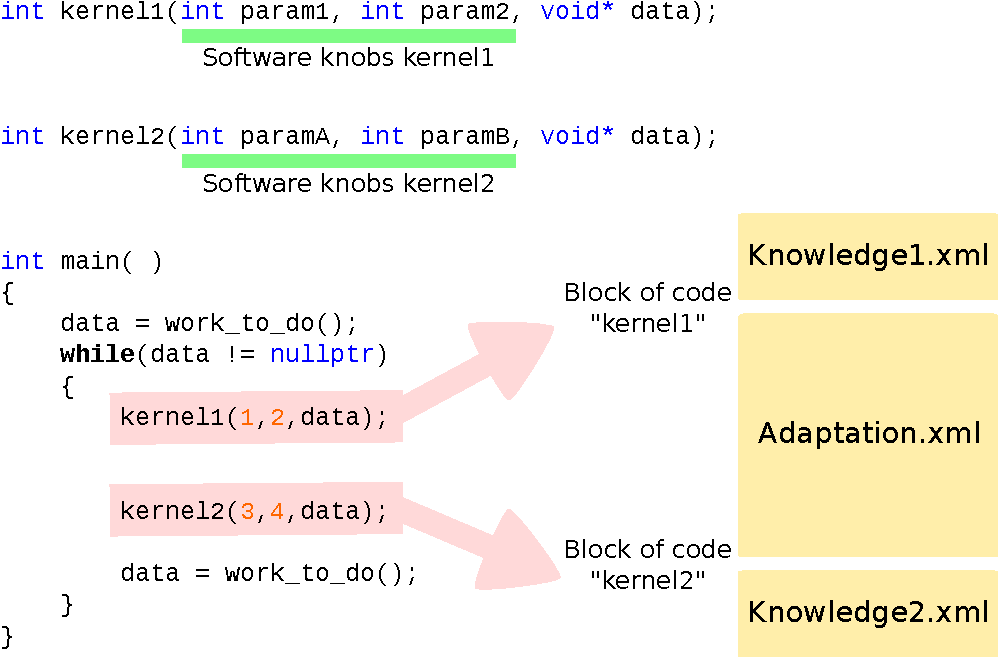
\includegraphics[scale=0.5]{code_example1}
\caption{Pseudo-code of an application with two block of code to be tuned.}
\label{fig:code_example1}
\end{figure}


To clarify the concept, \prettyref{fig:code_example1} shows a pseudo-code of a very simple application.
The whole computation is a loop that executes two different kernels on the same data.
In this example we suppose that the developer is interested on managing two different blocks of the application (highlighted in red).
The first block is named ``kernel1'', while the second block is named ''kernel2''.
We would like to stress the fact that a block of code might involve several lines of code, not just a function call.
In this case we have a single configuration file for the Monitor and Plan elements (\textit{Adaptation.xml}) of both the blocks of code; while we have two different files for the application Knowledge (\textit{Knowledge1.xml} and \textit{Knowledge2.xml}).
